\documentclass[11pt,a4paper]{article}
\usepackage[margin=1in]{geometry}
\usepackage[T1]{fontenc}
\usepackage[utf8]{inputenc}
\usepackage{lmodern}
\usepackage{hyperref}
\usepackage{enumitem}
\usepackage{xurl}
\usepackage{tikz}
\usepackage{float}
\usetikzlibrary{arrows.meta, positioning, shapes.geometric}
\hypersetup{colorlinks=true,linkcolor=blue,urlcolor=blue}
\newcommand{\codepath}[1]{\path{#1}}
\tikzset{box/.style={rectangle,draw,rounded corners,align=center,inner sep=3pt,minimum width=36mm},line/.style={-Latex}}

\title{Phase-1 Deliverable: Documentation}
\author{SIT Engine Architecture}
\date{\today}

\begin{document}
\maketitle

\section{Technical Description}
Documentation deliverable defines architecture, operational usage, and extension boundaries so contributors can implement safely without tribal knowledge.

It also records baseline provenance: Phase-0 implementation and parity reference came from the Tenstorrent Wormhole testbench.

\section{Implementation Fulfillment}
Primary paths: \codepath{Phase-1/README.md}, \codepath{Phase-1/docs/guides/GENERALIZATION.md}, \codepath{Phase-1/docs/phase1_technical_document.tex}, \codepath{Phase-1/docs/phase1_deliverables_matrix.tex}, plus validation/reference docs under \codepath{Phase-1/docs/}. Phase-0 conversion provenance is documented via \codepath{Phase-1/phase0_trace_to_sit.py}.

\subsection*{Phase-0 Baseline Provenance (Verified)}
\begin{itemize}[leftmargin=*]
  \item Source repo: \url{git@github.com:Srinidhi-Magesh08/Tenstorrent_test_raw_files.git}
  \item Baseline branch/commit: \texttt{main} @ \texttt{4512ce4e1a689f64c866160bf1f8e7e5e3e2ec89}
  \item Baseline run artifact: \codepath{phase0_golden/tt_run_2026-02-09/raw_profiler/profile_log_device.csv}
  \item Run header baseline: \texttt{ARCH=wormhole\_b0}, \texttt{CHIP\_FREQ[MHz]=1000}, \texttt{Max Compute Cores=64}
\end{itemize}

\section{Design \& Architecture}
Docs are partitioned by intent: onboarding guide, architecture/specification, runbooks, status tracking, and deliverable-specific technical references.

\subsection*{Function Flowchart}
\begin{figure}[H]
\centering
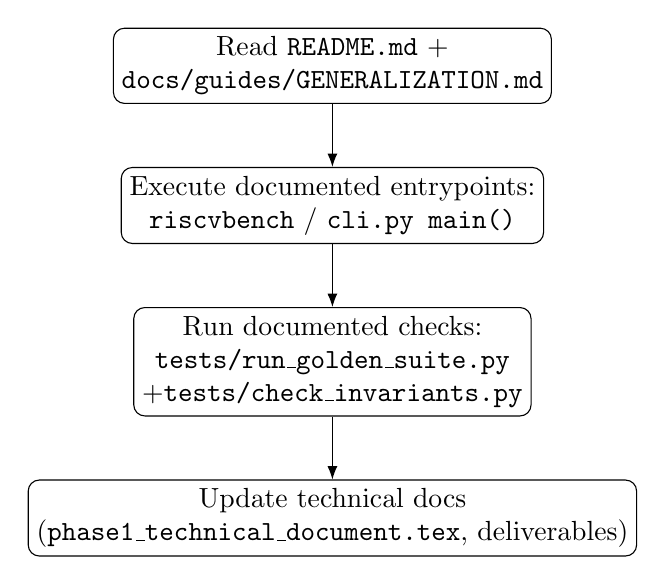
\begin{tikzpicture}[node distance=8mm and 12mm]
\node[box] (a) {Read \texttt{README.md} +\\\texttt{docs/guides/GENERALIZATION.md}};
\node[box, below=of a] (b) {Execute documented entrypoints:\\\texttt{riscvbench} / \texttt{cli.py main()}};
\node[box, below=of b] (c) {Run documented checks:\\\texttt{tests/run\_golden\_suite.py}\\+\texttt{tests/check\_invariants.py}};
\node[box, below=of c] (d) {Update technical docs\\(\texttt{phase1\_technical\_document.tex}, deliverables)};
\draw[line] (a) -- (b);
\draw[line] (b) -- (c);
\draw[line] (c) -- (d);
\end{tikzpicture}
\caption{Documentation Function Flow}
\end{figure}

\end{document}
